\documentclass{beamer}

%
% Choose how your presentation looks.
%
% For more themes, color themes and font themes, see:
% http://deic.uab.es/~iblanes/beamer_gallery/index_by_theme.html
%
\mode<presentation>
{
  \usetheme{default}      % or try Darmstadt, Madrid, Warsaw, ...
  \usecolortheme{default} % or try albatross, beaver, crane, ...
  \usefonttheme{default}  % or try serif, structurebold, ...
  \setbeamertemplate{navigation symbols}{}
  \setbeamertemplate{caption}[numbered]
  \setbeamertemplate{footline}[page number]
  \setbeamercolor{frametitle}{fg=white}
  \setbeamercolor{footline}{fg=black}
} 

\usepackage[english]{babel}
\usepackage[utf8x]{inputenc}
\usepackage{tikz}
\usepackage{listings}
\usepackage{courier}

\xdefinecolor{darkblue}{rgb}{0.1,0.1,0.7}
\xdefinecolor{dianablue}{rgb}{0.18,0.24,0.31}
\definecolor{commentgreen}{rgb}{0,0.6,0}
\definecolor{stringmauve}{rgb}{0.58,0,0.82}

\lstset{ %
  backgroundcolor=\color{white},      % choose the background color
  basicstyle=\ttfamily\scriptsize,         % size of fonts used for the code
  breaklines=true,                    % automatic line breaking only at whitespace
  captionpos=b,                       % sets the caption-position to bottom
  commentstyle=\color{commentgreen},  % comment style
  escapeinside={\%*}{*)},             % if you want to add LaTeX within your code
  keywordstyle=\color{blue},          % keyword style
  stringstyle=\color{stringmauve},    % string literal style
  showstringspaces=false,
  showlines=true
}

\lstdefinelanguage{scala}{
  morekeywords={abstract,case,catch,class,def,%
    do,else,extends,false,final,finally,%
    for,if,implicit,import,match,mixin,%
    new,null,object,override,package,%
    private,protected,requires,return,sealed,%
    super,this,throw,trait,true,try,%
    type,val,var,while,with,yield},
  otherkeywords={=>,<-,<\%,<:,>:,\#,@},
  sensitive=true,
  morecomment=[l]{//},
  morecomment=[n]{/*}{*/},
  morestring=[b]",
  morestring=[b]',
  morestring=[b]"""
}

\lstdefinelanguage{cpp}{
  morekeywords={for,if,class,public,typedef,struct,double,return,Int_t,int,void,Long64_t},
  otherkeywords={=>,<-,<\%,<:,>:,\#,@},
  sensitive=true,
  morecomment=[l]{//},
  morecomment=[n]{/*}{*/},
  morestring=[b]",
  morestring=[b]',
  morestring=[b]"""
}

\title[2016-07-28-root-jit]{Python-based histogramming as fast as C++}
\author{Jim Pivarski}
\institute{Princeton University -- DIANA}
\date{July 28, 2016}

\begin{document}

\logo{\pgfputat{\pgfxy(0.11, 8)}{\pgfbox[right,base]{\tikz{\filldraw[fill=dianablue, draw=none] (0 cm, 0 cm) rectangle (50 cm, 1 cm);}}}\pgfputat{\pgfxy(0.11, -0.6)}{\pgfbox[right,base]{\tikz{\filldraw[fill=dianablue, draw=none] (0 cm, 0 cm) rectangle (50 cm, 1 cm);}
\includegraphics[height=0.99 cm]{diana-hep-logo.png}\tikz{\filldraw[fill=dianablue, draw=none] (0 cm, 0 cm) rectangle (4.9 cm, 1 cm);}}}}

\begin{frame}
  \titlepage
\end{frame}

\logo{\pgfputat{\pgfxy(0.11, 8)}{\pgfbox[right,base]{\tikz{\filldraw[fill=dianablue, draw=none] (0 cm, 0 cm) rectangle (50 cm, 1 cm);}
\includegraphics[height=1 cm]{diana-hep-logo.png}}}}

% Uncomment these lines for an automatically generated outline.
%\begin{frame}{Outline}
%  \tableofcontents
%\end{frame}

\begin{frame}{Start with the punchline}
\vspace{0.25 cm}
Wall time to fill 100-bin histogram with {\tt \small 2*x}, selecting on {\tt \small !y}.

TTree has 1 million entries, fully loaded into TTreeCache.

\renewcommand{\arraystretch}{1.2}
\vspace{0.25 cm}
\begin{tabular}{l c c c c}
\textcolor{darkblue}{ROOT} & & & & \\
Fill method & Preparation & Prep (ms) & Run (ms) & Relative \\\hline
C++ & compilation & 12.6 & \textcolor{red}{198} & \textcolor{red}{1} \\
PyROOT & none & & 15,700 & 79 \\
TFormula & first pass & 380 & 317 & 1.6\vspace{0.25 cm} \\
\textcolor{darkblue}{Histogrammar} & & & & \\
Fill method & Preparation & Prep (ms) & Run (ms) & Relative \\\hline
pure Python & none & & 21,000 & 105 \\
with Numpy & first pass & 814 & 312 & 1.6 \\
with ROOT & JIT-compilation & 219 & \textcolor{red}{196} & \textcolor{red}{0.98} \\
\end{tabular}
\end{frame}

\begin{frame}[fragile]{ROOT code in the test}

\vspace{0.3 cm}
\hfill \textcolor{darkblue}{C++ ROOT}

\vspace{-0.5 cm}
\begin{minipage}{0.8\linewidth}
\begin{lstlisting}[language=cpp]
TH1D control1("control1", "", 100, -10, 10);
// start stopwatch
ttree->SetBranchAddress("x", &input_x);
ttree->SetBranchAddress("y", &input_y);
for (i = 0;  i < ttreeEntries;  ++i) {
  root_ttree->GetEntry(i);
  if (!input_y)
    control1.Fill(2 * input_x);
}
// end stopwatch
\end{lstlisting}
\end{minipage}

\hfill \textcolor{darkblue}{PyROOT}

\vspace{-0.5 cm}
\begin{minipage}{0.8\linewidth}
\begin{lstlisting}[language=python]
control2 = ROOT.TH1D("control2", "", 100, -10, 10)
# start stopwatch
for entry in root_ttree:
    if not entry.y:
        control2.Fill(2 * entry.x)
# end stopwatch
\end{lstlisting}
\end{minipage}

\hfill \textcolor{darkblue}{TFormula}

\vspace{-0.5 cm}
\begin{minipage}{0.8\linewidth}
\begin{lstlisting}[language=python]
control3 = ROOT.TH1D("control3", "", 100, -10, 10)
# start stopwatch
root_ttree.Draw("2 * x >>+ control3", "!y", "goff")
# end stopwatch
\end{lstlisting}
\end{minipage}
\end{frame}

\begin{frame}[fragile]{Histogrammar code in the test}
\vspace{0.3 cm}

\hfill \textcolor{darkblue}{pure Python}

\vspace{-0.5 cm}
\begin{minipage}{0.8\linewidth}
\begin{lstlisting}[language=python]
experiment1 = Select(lambda t: not t.y,
                  Bin(100, -10, 10,
                      lambda t: 2 * t.x))
# start stopwatch
for t in list_of_entries:
    experiment1.fill(t)
# end stopwatch
\end{lstlisting}
\end{minipage}

\vspace{0.5 cm}
\hfill \textcolor{darkblue}{with Numpy}

\vspace{-0.5 cm}
\begin{minipage}{0.8\linewidth}
\begin{lstlisting}[language=python]
experiment2 = Select("logical_not(y)",
\end{lstlisting}
\end{minipage}

\vspace{-0.45 cm}
\begin{minipage}{\linewidth}
\begin{lstlisting}[language=python]
                  Bin(100, -10, 10, "2 * x"))
# start stopwatch
experiment2.numpy(dict_of_numpy_arrays)
# end stopwatch
\end{lstlisting}
\end{minipage}

\vspace{0.5 cm}
\hfill \textcolor{darkblue}{with ROOT}

\vspace{-0.5 cm}
\begin{minipage}{0.8\linewidth}
\begin{lstlisting}[language=python]
experiment3 = Select("!y",
\end{lstlisting}
\end{minipage}

\vspace{-0.45 cm}
\begin{minipage}{\linewidth}
\begin{lstlisting}[language=python]
                  Bin(100, -10, 10, "2 * x"))
# start stopwatch
experiment3.cling(root_ttree)
# end stopwatch
\end{lstlisting}
\end{minipage}
\end{frame}

\begin{frame}{}
\begin{center}
\textcolor{darkblue}{\Large Back to the beginning for some context}
\end{center}
\end{frame}

\begin{frame}[fragile]{Grammar of histograms}
\vspace{0.5 cm}
\begin{center}

\includegraphics[width=0.5\linewidth]{histogrammar-logo.png}
\end{center}

\textcolor{darkblue}{A suite of classes that each aggregate a simple thing and can aggregate complex things when combined.}

\vspace{0.35 cm}
For instance, an ordinary histogram is

\begin{lstlisting}[language=python]
histogram = Bin(10, -5, 5, "pt", Count())
\end{lstlisting}

and a histogram with {\tt\small Sumw2} is

\begin{lstlisting}[language=python]
histogram = Bin(10, -5, 5, "pt", Branch(Count(), Count("x**2")))
\end{lstlisting}

The content in each bin is now a count {\it and} a sum of weights squared.

\begin{center}
\textcolor{darkblue}{\url{http://histogrammar.org}}
\end{center}
\end{frame}

\begin{frame}{Catalog of primitives}

\vspace{0.5 cm}
\begin{columns}
\column{0.45\linewidth}
\textcolor{darkblue}{\bf Count:} sum of weights \\
\textcolor{darkblue}{\bf Sum:} sum of anything \\
\textcolor{darkblue}{\bf Average:} average \\
\textcolor{darkblue}{\bf Deviate:} average and variance (for a profile plot) \\
\textcolor{darkblue}{\bf Minimize:} minimum value \\
\textcolor{darkblue}{\bf Maximize:} maximum value \\
\textcolor{darkblue}{\bf Fraction:} ratio of contents (for an efficiency plot) \\
\textcolor{darkblue}{\bf Stack:} cumulative filling \\
\textcolor{darkblue}{\bf Select:} apply a cut \\
\textcolor{darkblue}{\bf Limit:} drop detail when large

\column{0.6\linewidth}
\textcolor{darkblue}{\bf Bin:} regular binning (normal histogram) \\
\textcolor{darkblue}{\bf SparselyBin:} bins in a hashmap \\
\textcolor{darkblue}{\bf CentrallyBin:} irregular bins defined by the centers of each bin \\
\textcolor{darkblue}{\bf IrregularlyBin:} \ldots defined by edges \\
\textcolor{darkblue}{\bf Categorize:} bin unique by string value (bar chart as a kind of histogram) \\
\textcolor{darkblue}{\bf Label:} directory with string-based keys \\
\textcolor{darkblue}{\bf UntypedLabel:} no type restrictions \\
\textcolor{darkblue}{\bf Index:} homogeneous list \\
\textcolor{darkblue}{\bf Branch:} heterogeneous tuple \\
\textcolor{darkblue}{\bf Bag:} accumulate raw data (scatter) \\
\end{columns}

\vspace{0.25 cm}
\begin{itemize}
\item All are one-pass, commutative, and associative (parallelizable).
\item Implement in Python, Scala, \textcolor{gray}{Julia, C++,} \textcolor{lightgray}{R, Javascript\ldots}
\item Back-ends for filling, front-ends for plotting, including ROOT.
\end{itemize}
\end{frame}

\begin{frame}[fragile]{Using ROOT as a back-end}
When a user types

\begin{center}
\begin{minipage}{0.9\linewidth}
\begin{lstlisting}[language=python, basicstyle=\ttfamily\small]
h = Select("!y", Bin(100, -10, 10, "2 * x"))
h.cling(root_ttree)
\end{lstlisting}
\end{minipage}
\end{center}

Histogrammar-Python generates C++ code

\begin{itemize}
\item for this specific combination ({\tt\small Select-Bin-Count}),
\item for this specific TTree,
\item with these derived fields.
\end{itemize}

and sends it to Cling to compile and run.
\end{frame}

\begin{frame}[fragile]{}
\vspace{1 cm}

\Large The code generated by this example

\vspace{0.25 cm}
\begin{columns}
\column{0.35\linewidth}
\begin{lstlisting}[language=cpp, basicstyle=\ttfamily\fontsize{5}{4}\selectfont]
class HistogrammarClingFiller_0 {
public:
  typedef struct {
    double entries;
    double underflow;
    double overflow;
    double nanflow;
    double values[100];
    double& getValues(int i) { return values[i]; }
  } Bn100CtCtCtCt;

  typedef struct {
    double entries;
    Bn100CtCtCtCt cut;
  } SeBn100CtCtCtCt;

  double weight_0;
  double weight_1;
  Int_t input_y;
  double input_x;
  double quantity_0;
  double quantity_1;
  int bin_0;
  SeBn100CtCtCtCt storage;

  void fillall(TTree* ttree, Long64_t start, Long64_t end) {
    storage.entries = 0.0;
    storage.cut.entries = 0.0;
\end{lstlisting}

\column{0.35\linewidth}
\begin{lstlisting}[language=cpp, basicstyle=\ttfamily\fontsize{5}{4}\selectfont]
    storage.cut.nanflow = 0.0;
    storage.cut.underflow = 0.0;
    storage.cut.overflow = 0.0;
    for (bin_0 = 0;  bin_0 < 100;  ++bin_0) {
      storage.cut.values[bin_0] = 0.0;
    }
    weight_0 = 1.0;
    ttree->SetBranchAddress("x", &input_x);
    ttree->SetBranchAddress("y", &input_y);

    if (start < 0) start = 0;
    if (end < 0) end = ttree->GetEntries();
    for (;  start < end;  ++start) {
      ttree->GetEntry(start);
      quantity_0 = !input_y;
      quantity_1 = 2 * input_x;
      storage.entries += weight_0;
      if (!isnan(quantity_0)  &&  quantity_0 > 0.0) {
        weight_1 = weight_0 * quantity_0;
\end{lstlisting}

\column{0.35\linewidth}
\begin{lstlisting}[language=cpp, basicstyle=\ttfamily\fontsize{5}{4}\selectfont]
        storage.cut.entries += weight_1;
        if (isnan(quantity_1)) {
          storage.cut.nanflow += weight_1;
        }
        else if (quantity_1 < -10.0) {
          storage.cut.underflow += weight_1;
        }
        else if (quantity_1 >= 10.0) {
          storage.cut.overflow += weight_1;
        }
        else {
          bin_0 = floor((quantity_1 - -10.0) * 5.0);
          storage.cut.values[bin_0] += weight_1;
        }
      }
    }

    ttree->ResetBranchAddresses();
  }
};
\end{lstlisting}
\end{columns}
\end{frame}

\begin{frame}{Properties of this code}

\begin{itemize}\setlength{\itemsep}{0.35 cm}
\item Arbitrarily deep nesting: any aggregator that can be constructed out of primitives generates working C++ code.
\item Human-readable for debugging, with good indentation.
\item All but three primitives ({\tt\small SparselyBin}, {\tt\small Categorize}, {\tt\small Bag}) generate {\it memory-contiguous} code, and nothing is allocated in the loop (not even on the stack). Expect good CPU caching.
\item Repeated expressions are computed once and reused.
\item Expressions are sanitized, with code-transformations applied to the abstract syntax tree (AST), not raw strings.
\end{itemize}
\end{frame}

\begin{frame}{What this means for analysis}

\vspace{0.5 cm}
\textcolor{darkblue}{Python users can turn TTrees into TCanvases at C++ speeds.}

\begin{itemize}
\item They have to describe their aggregation in terms of this 20-primitive language.
\begin{itemize}
\item like a generalization of TFormula
\item but whole directories of histograms can be filled in one pass
\end{itemize}
\item They have to write their ``fill rules'' as declarative C99 expressions with TTree branches as free variables.
\begin{itemize}
\item dealing with bad identifier: {\tt\small "t($\backslash$"branch-name$\backslash$") + 3"}
\item multi-line returns last statement: {\tt\small "auto tmp = init(); while (tmp.next()); tmp.value()"}
\item derived quantities can be written globally for all fill rules \\ (e.g. find the leading jet once, use it in all rules).
\item can still load C++ libraries for more complex functions
\end{itemize}
\item Aliases exist to make some composites more familiar:

{\tt\small Profile(n, low, high, xRule, yRule, cutRule)}

\item {\tt\small .cling(...)} fills with TTrees, {\tt\small .root(...)} returns TH1, TProfile, TH2, TEfficiency, etc.
\end{itemize}
\end{frame}

\begin{frame}[fragile]{Whole analysis example}
\vspace{0.1 cm}
\begin{lstlisting}[language=python]
from ROOT import *; from histogrammar import *             
gInterpreter.AddIncludePath("Event.h")         # works for
gInterpreter.ProcessLine(".L Event.cxx")       # complex events
tfileData = TFile("data.root"); data = tfileEvent.Get("Events")
tfileMC1 = TFile("mc1.root"); mc1 = tfileEvent.Get("Events")
tfileMC2 = TFile("mc2.root"); mc2 = tfileEvent.Get("Events")

plots = UntypedLabel(           # book all aggregators together
    mass = Bin(100, 0, 50, "event.dijet.mass()"),  # quoted C++
    pt =   Bin(100, 0, 300, "event.dijet.pt()"),      # hist
    profile = Bin(100, 0, 300, "event.dijet.pt()",    # prof
                  Deviate("event.dijet.eta()")),
    twodim =  Bin(100, 0, 300, "event.dijet.pt()",    # 2D
                  Bin(100, -5, 5, "event.dijet.eta()")),
    trigeff = Fraction("trigger",                     # eff
                  Bin(100, 0, 300, "event.maxjet.pt()")))

plotsData = plots.copy().cling(data)   # fill all at once
plotsMC1 = plots.copy().cling(mc1)     # for each sample
plotsMC2 = plots.copy().cling(mc2)

tefficiency = plotsData.get("trigeff").root("efficiency vs pt")
tefficiency.Draw()
tstack = Stack.build(plotsMC1.get("mass"), plotsMC2.get("mass"))
tstack.root("backgrounds").Draw()      # get ordinary ROOT plots
\end{lstlisting}
\end{frame}

\begin{frame}{Wishlist}
\vspace{0.5 cm}
Histogrammar-Cling is complete (with tests) for all primitives in {\tt\small histogrammar-python/master}.

\setlength{\itemsep}{0.5 cm}
\begin{itemize}
\item However, it only operates on TTree; should at least generalize to TChain.
\item Better still, it should make use of Enric's parallel reading to escape the Python GIL (one call from Python would dispatch threads on the C++ side).
\item Moreover, it's a natural fit for the ``chains of functional primitives.'' All of Histogrammar's primitives are glorified reducers. Map, filter, and flatMap would greatly expand capabilities.
\item Proposal/request: add Histogrammar as a part of PyROOT?
\begin{itemize}
\item pure Python; 2.6 (SL6), 2.7, 3.4 continuously tested
\item no explicit dependencies (import statements are hidden)
\end{itemize}
\end{itemize}
\end{frame}

\begin{frame}[fragile]{Last slide: possible inclusion in ROOT}
\vspace{0.25 cm}
Just the Python implementation, latest version for a some release of the Histogrammar specification (e.g. 0.9.x or 1.0.x).

\begin{center}
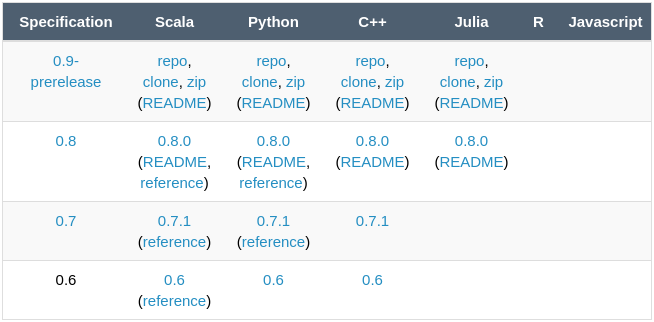
\includegraphics[width=0.75\linewidth]{release_matrix.png}
\end{center}

Nested under {\tt\small import ROOT}, so that user can also install it standalone for another version, distinguishing namespaces as

\hfill\begin{minipage}{0.95\linewidth}
\begin{lstlisting}{language=python}
import ROOT.histogrammar as hg09
import histogrammar as hg10
\end{lstlisting}
\end{minipage}

\vfill
Target an upcoming ROOT 6 release, rather than ROOT 7?
\end{frame}

\begin{frame}[fragile]{Backup: why not this syntax?}

\vspace{0.5 cm}
\fbox{\tt\small root\_tree.Filter("!y").Map("2*x").Bin(100, -10, 10)}

\vspace{0.2 cm}
The ``chains of functional primitives'' should implement {\tt Filter} and {\tt Map} as above. These are different from Histogrammar's primitives.

\begin{itemize}
\item Histogrammar has its own {\tt Select} because it applies different cuts to different parts of the aggregation tree.
\item Histogrammar primitives have their own fill rules (rather than relying on an upstream {\tt Map}) because they are projections of complex events onto plotable number lines.
\item So you can do this:
\end{itemize}

\begin{minipage}{1.05\linewidth}
\begin{lstlisting}[language=python, basicstyle=\ttfamily\scriptsize]
functional_chains.Histogrammar(UntypedLabel(
    plot1 = Select("jet.pt > 20", Bin(100, -5, 5, "muon.pt")),
    plot2 = Bin(10, 0, 100, "jet.pt", Bin(10, -5, 5, "muon.pt")),
    frac = Fraction("trigger", Bin(100, 0, 100, "jet.pt")),
    weirdo = Branch(..., Select(...)),
    ...
    ))
\end{lstlisting}
\end{minipage}
\end{frame}

\begin{frame}{Backup: time is dominated by TTree-reading}
\vspace{0.5 cm}
\renewcommand{\arraystretch}{1.2}
\begin{tabular}{l c}
ROOT C++ with TTree read and histogram fill & 198 ms \\
ROOT C++ filling histogram with zeros & 25 ms \\
C++ empty for loop & 5 ms \\
 & \\
Histogrammar-Cling with TTree read and histogram fill & 196 ms \\
Histogrammar-Cling filling histogram with zeros & 19 ms \\
C++ empty for loop & 5 ms \\
\end{tabular}

\vspace{1 cm}
ROOT C++ and Histogrammar-Cling filling times are nearly the same because they both call {\tt\small ttree->GetEntry(i)}, which takes 90\% of the time.
\end{frame}

\begin{frame}[fragile]{Backup: TTreeCache is enabled}
\scriptsize
\begin{lstlisting}
TFile::PrintCacheStats()

******TreeCache statistics for tree: big in file: test/big.root ******
Number of branches in the cache ...: 2
Cache Efficiency ..................: 1.000000
Cache Efficiency Rel...............: 1.000000
Learn entries......................: 100
Cached Reading.....................: 8022693 bytes in 1 transactions
Reading............................: 0 bytes in 0 uncached transactions
Readahead..........................: 256000 bytes with overhead = 0 bytes
Average transaction................: 8022.693000 Kbytes
Number of blocks in current cache..: 377, total size: 8022693

These values were constant throughout the test:
    TFile::GetBytesRead() = 8031424
    TFile::GetReadCalls() = 5
\end{lstlisting}
\end{frame}

\end{document}

%% TFile::PrintCacheStats()

%% ******TreeCache statistics for tree: big in file: test/big.root ******
%% Number of branches in the cache ...: 2
%% Cache Efficiency ..................: 1.000000
%% Cache Efficiency Rel...............: 1.000000
%% Learn entries......................: 100
%% Cached Reading.....................: 8022693 bytes in 1 transactions
%% Reading............................: 0 bytes in 0 uncached transactions
%% Readahead..........................: 256000 bytes with overhead = 0 bytes
%% Average transaction................: 8022.693000 Kbytes
%% Number of blocks in current cache..: 377, total size: 8022693

%% These values were constant throughout the test:
%%     TFile::GetBytesRead() = 8031424
%%     TFile::GetReadCalls() = 5

%% line |
%%    1 | class HistogrammarClingFiller_0 {
%%    2 | public:
%%    3 |
%%    4 |   typedef struct {
%%    5 |     double entries;
%%    6 |     double underflow;
%%    7 |     double overflow;
%%    8 |     double nanflow;
%%    9 |     double values[100];
%%   10 |     double& getValues(int i) { return values[i]; }
%%   11 |   } Bn100CtCtCtCt;
%%   12 |
%%   13 |   typedef struct {
%%   14 |     double entries;
%%   15 |     Bn100CtCtCtCt cut;
%%   16 |   } SeBn100CtCtCtCt;
%%   17 |
%%   18 |   double weight_0;
%%   19 |   double weight_1;
%%   20 |   Int_t input_boolean;
%%   21 |   double input_noholes;
%%   22 |
%%   23 |   double quantity_0;
%%   24 |   double quantity_1;
%%   25 |   int bin_0;
%%   26 |   SeBn100CtCtCtCt storage;
%%   27 |
%%   28 |   bool isnan(double x) { return x != x; }
%%   29 |   bool isnan(float x) { return x != x; }
%%   30 |   bool isnan(int x) { return false; }
%%   31 |
%%   32 |   void fillall(TTree* ttree, Long64_t start, Long64_t end) {
%%   33 |     storage.entries = 0.0;
%%   34 |     storage.cut.entries = 0.0;
%%   35 |     storage.cut.nanflow = 0.0;
%%   36 |     storage.cut.underflow = 0.0;
%%   37 |     storage.cut.overflow = 0.0;
%%   38 |     for (bin_0 = 0;  bin_0 < 100;  ++bin_0) {
%%   39 |       storage.cut.values[bin_0] = 0.0;
%%   40 |     }
%%   41 |     weight_0 = 1.0;
%%   42 |     ttree->SetBranchAddress("noholes", &input_noholes);
%%   43 |     ttree->SetBranchAddress("boolean", &input_boolean);
%%   44 |
%%   45 |     if (start < 0) start = 0;
%%   46 |     if (end < 0) end = ttree->GetEntries();
%%   47 |     for (;  start < end;  ++start) {
%%   48 |       ttree->GetEntry(start);
%%   49 |       quantity_0 = !input_boolean;
%%   50 |       quantity_1 = 2 * input_noholes;
%%   51 |       storage.entries += weight_0;
%%   52 |       if (!isnan(quantity_0)  &&  quantity_0 > 0.0) {
%%   53 |         weight_1 = weight_0 * quantity_0;
%%   54 |         storage.cut.entries += weight_1;
%%   55 |         if (isnan(quantity_1)) {
%%   56 |           storage.cut.nanflow += weight_1;
%%   57 |         }
%%   58 |         else if (quantity_1 < -10.0) {
%%   59 |           storage.cut.underflow += weight_1;
%%   60 |         }
%%   61 |         else if (quantity_1 >= 10.0) {
%%   62 |           storage.cut.overflow += weight_1;
%%   63 |         }
%%   64 |         else {
%%   65 |           bin_0 = floor((quantity_1 - -10.0) * 5.0);
%%   66 |           storage.cut.values[bin_0] += weight_1;
%%   67 |         }
%%   68 |       }
%%   69 |     }
%%   70 |
%%   71 |     ttree->ResetBranchAddresses();
%%   72 |   }
%%   73 | };

%% class ControlTest {
%% public:
%%   TH1D histogram;
%% 
%%   ControlTest() : histogram("control1", "", 100, -10, 10) {}
%% 
%%   Int_t input_boolean;
%%   double input_noholes;
%% 
%%   void fillall(TTree* ttree, Long64_t start, Long64_t end) {
%%     if (start < 0) start = 0;
%%     if (end < 0) end = ttree->GetEntries();
%% 
%%     ttree->SetBranchAddress("noholes", &input_noholes);
%%     ttree->SetBranchAddress("boolean", &input_boolean);
%% 
%%     for (;  start < end;  ++start) {
%%       ttree->GetEntry(start);
%% 
%%       if (!input_boolean)
%%         histogram.Fill(2 * input_noholes);
%%     }
%% 
%%     ttree->ResetBranchAddresses();
%%   }
%% };

%% histogram = ROOT.TH1D("control2", "", 100, -10, 10)
%% for row in TestRootCling.ttreeBig:
%%     if not row.boolean:
%%         histogram.Fill(2 * row.noholes)

%% Histogrammar JIT-compilation
%% 0.21904706955 -> 1.1003578233905158

%% Histogrammar running
%% 0.196442842484 -> 0.9868080820273187
%% 0.195878982544 -> 0.9839755963083809
%% 0.19778585434 -> 0.9935545480069445

%% Histogrammar running without ttree->GetEntry(i) (fill with zeros)
%% 0.0193800926208 -> 0.09735367187125231
%% 0.0191719532013 -> 0.09630810737649194
%% 0.019119977951 -> 0.09604701566954614

%% Completely empty loop (in the Histogrammar test)
%% 0.00551819801331 -> 0.02772003463656316
%% 0.00556516647339 -> 0.027955975307250087
%% 0.00550293922424 -> 0.027643383860256804

%% ROOT C++ compilation
%% 0.0126299858093 -> 0.06344528471951177

%% ROOT C++ first event
%% 0.0141220092773 -> 0.07094029343644556

%% ROOT C++ subsequent
%% 0.198187828064 -> 0.995573816892438
%% 0.19960808754 -> 1.0027083274287882
%% 0.199410915375 -> 1.0017178556787742

%% ROOT C++ subsequent without ttree->GetEntry(i) (fill with zeros)
%% 0.0239660739899 -> 0.12039082314553802
%% 0.0246810913086 -> 0.12398263061462476
%% 0.0245039463043 -> 0.1230927630087422

%% Completely empty loop (in the ROOT C++ test)
%% 0.00520300865173 -> 0.026136717039224343
%% 0.00507307052612 -> 0.02548398777256311
%% 0.00515604019165 -> 0.025900776368537416

%% PyROOT first event
%% 0.00721597671509 -> 0.03624863116482206

%% PyROOT subsequent
%% 15.7434358597 -> 79.08534385260707
%% 15.7216258049 -> 78.97578354450955
%% 15.6935698986 -> 78.83484791796619

%% TFormula first pass
%% 0.379606962204 -> 1.9069120236704813

%% TFormula subsequent
%% 0.317915201187 -> 1.597010539878666
%% 0.316998958588 -> 1.5924079002998555
%% 0.316241025925 -> 1.588600512522203

%% Numpy first
%% 0.814823865891 -> 4.093174208449328

%% Numpy subsequent
%% 0.309661865234 -> 1.5555508535947518
%% 0.312314987183 -> 1.5688785073222755
%% 0.313981056213 -> 1.5772478139522859

%% Native Histogrammar

%% Native first
%% 20.7954871655 -> 104.4637439833533

%% Native subsequent
%% 21.058177948 -> 105.78334099165966
%% 20.9882600307 -> 105.43211635553794
%% 20.9792170525 -> 105.38668999201907
